\hypertarget{group__usecase2}{}\section{Use case 2}
\label{group__usecase2}\index{Use case 2@{Use case 2}}
Collaboration diagram for Use case 2\+:\nopagebreak
\begin{figure}[H]
\begin{center}
\leavevmode
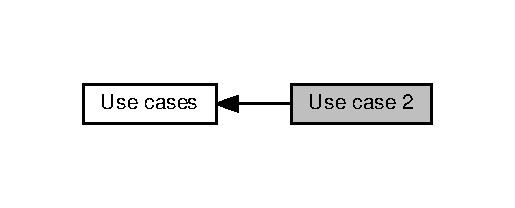
\includegraphics[width=247pt]{group__usecase2}
\end{center}
\end{figure}
Or one can use demo loader with a simple command interpreter.  
\begin{DoxyCode}
    \hyperlink{struct_camera}{Camera} camera;
camera.\hyperlink{struct_camera_ab0cbf1b102afdeb285ef2be271d1701c}{resolution}(960, 540, 36.87, 0.5);
std::unique\_ptr<Pipeline> pipeline( \textcolor{keyword}{new} \hyperlink{class_mesh_transformation}{MeshTransformation}());
pipeline->translate( make\_float3(0,0,10));
pipeline->scale( make\_float3(1,1,1) );
camera.modelDir = pipeline->transform() * defaultCameraMatrix.inverse();
camera.modelOrig = camera.modelDir;

\textcolor{comment}{//set lights}
std::vector<ILight> lights;
std::unique\_ptr<Pipeline> light\_pipeline( \textcolor{keyword}{new} \hyperlink{class_mesh_transformation}{MeshTransformation}());

\hyperlink{class_square_matrix4}{SquareMatrix4f} l2w(0.95292, 0.289503, 0.0901785, 0,
     -0.0960954, 0.5704, -0.815727, 0,
     -0.287593, 0.768656, 0.571365, 0,
         0, 0, 0, 1);
light\_pipeline->translate( make\_float3(0,0,5));
\textcolor{comment}{//lights.push\_back( ILight( l2w, Vec3f(1, 1, 1), 1.0f, DISTANT\_LIGHT) );}
lights.push\_back( \hyperlink{class_i_light}{ILight}( l2w, \hyperlink{class_vec3}{Vec3f}(1, 1, 1), 1.0f, DISTANT\_LIGHT) );
lights.push\_back( \hyperlink{class_i_light}{ILight}( light\_pipeline->transform()*l2w, \hyperlink{class_vec3}{Vec3f}(1, 1, 1), 1.0f, DISTANT\_LIGHT) 
      );
\textcolor{comment}{//Special constructor with demo launch.}
\hyperlink{class_geometry_loader}{GeometryLoader<Mesh, Boundaries>} loader(lights);
\end{DoxyCode}
 